\section{Causal Graphs}

\subsection{An Overview}
\label{sec:graph-overview}
The previous section, \ref{sec:graph-importance}, motivated why the knowledge encoded in one's DAG is important.
This section gives a high level overview of what DAGs are and provides references for more thorough readings on the subject.
Causal diagrams and causal graphical models have been introduced by \citet{pearl_1995_causal} as a powerful tool for causal inference, especially in observational studies.
Perhaps one of the most important and useful features of causal
graphs when dealing with causal inference problems is the clear illustration
of the causal relationships between the variables.
While a formal introduction to the topic of DAGs is beyond the scope of this chapter,
here we focus specifically on illustrating the power of DAGs to represent
and encode complex causal relationships between variables in an intuitive and
clear manner.
Interested readers can refer to \citet{pearl_causality_2000} for a thorough introduction.

Consider the causal graph represented in Figure \ref{fig:simple-graph}.
Suppose we're interested in the effect of a treatment Z on Y.
What the graph in Figure \ref{fig:simple-graph} implies is that Z is
independent of Y(Z) given X.
For more information on how to semantically parse a causal graph as just done, see \citet[Ch 11.1]{pearl_2009_causality}.
Continuing with interpretation, in causal jargon, we say the mechanism by which the treatment Z was assigned is ignorable, once we control for covariates X.
In such situations, it is sufficient to control for X to obtain an unbiased estimate of the causal effect of Z on Y.

\begin{figure}[h!]
   \centering
   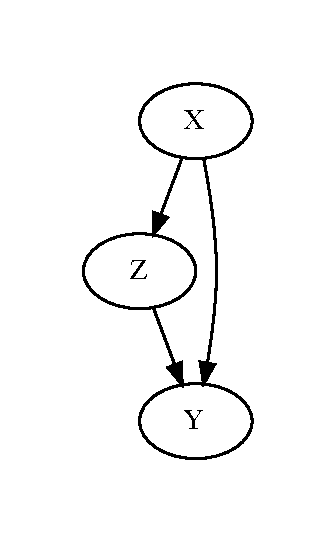
\includegraphics[height=0.25\textwidth]{simple-graph.pdf}
   \caption{Simple DAG of the causal relationships between X, Y and Z}
   \label{fig:simple-graph}
\end{figure}

The graph in Figure \ref{fig:simple-graph} can also be summarized by the following set of structural equations:
\[Z = f_Z(X, \epsilon_Z)  \]

\[Y(z) = f_Y(X, z, \epsilon_Y)  \]

Now consider the case where there exists another latent confounding variable, U, which also affects both the treatment Z, as well as the outcome, Y.
Figure \ref{fig:simple-graph-confounded} illustrates this assumption in DAG form, and the equations below are the structural equation equivalent:

\[Z = f_Z(X, U, \epsilon_Z)  \]

\[Y(z) = f_Y(X, U, z, \epsilon_Y)  \]

\begin{figure}[h!]
   \centering
   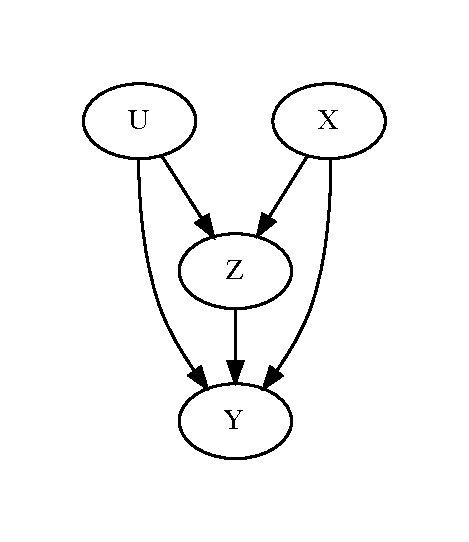
\includegraphics[height=0.25\textwidth]{simple-graph-confounded.pdf}
   \caption{Simple DAG of the causal relationships between X, Y, Z and confounder U}
   \label{fig:simple-graph-confounded}
\end{figure}

Figure \ref{fig:simple-graph-confounded} shows an indirect connection between Z and Y that goes through U.
Therefore, even if we condition on X, omitting U will yield biased results of the relationship between Z and Y, due to the variation in both Z and Y caused by U.
The structural equations also show that the ignorability assumption of Z does not hold if we only control for X, and we risk obtaining biased estimates of the causal effect of Z on Y if we fail to account for U, sometimes referred to as a common cause.
While the set of structural equations and the DAGs illustrate the same points in theory, the clarity of structural equations scales poorly with a problem's complexity.
As the number of covariates in one's causal system increases, a graphical representation of the relationship between those covariates quickly becomes more intuitive and easier to follow.
More importantly, graphically illustrating our assumptions eases the communication of these assumptions to the reader.
This communication is key to avoiding the misuse of our models in real-world applications.
For example, consider travel demand modelling applications.
Here, the communication advantage of DAGs is of particular relevance, as travel demand models typically involve many variables with complex interdependencies.

Another benefit of DAGs is that they come with testable implications.
Incorporating these tests in any causal analysis adds robustness and defensibility to one's study.
In section 5, we discuss these implications further, and we illustrate how to tests for them in one's analysis.

Lastly, it is important to note that the graphical approach to causality focuses
primarily on issues of identification of causal effects, as opposed to issues of estimation and inference. That is, given a
DAG that encodes an analyst's knowledge and assumptions about the data generation process of the problem at hand, one can determine algorithmically whether a causal effect of interest can be identified.
As such, we emphasize that DAGs are great tools
for a modeller to encode their assumptions about a problem.
Later on, we will use more familiar statistical tools to actually infer/estimate our causal effects of interest.

\subsection{Prior Uses of Causal Graphs in Choice Modelling}
\label{sec:choice-graphs}

In our last subsection, we reviewed the basics of causal graphs: what are they and why are they useful?
We targeted that subsection at choice modellers who are unfamiliar with these tools.
However, readers should be aware of the history of causal graphs in choice modelling.
Indeed, choice modellers have used causal graphs (in limited fashion) for years.
Here are three examples to illustrate our point.
First, consider the case of Random Utility Maximization (RUM) models.

\begin{figure}
   \centering
   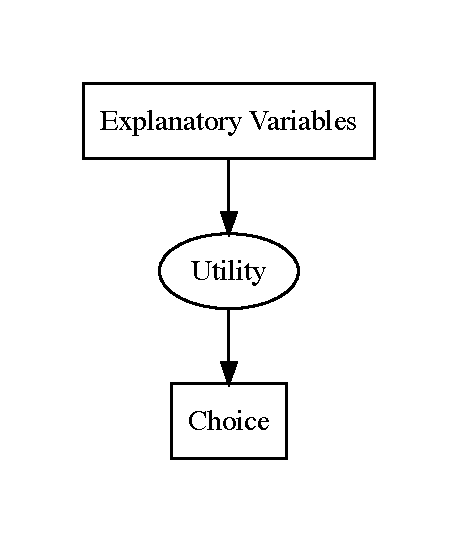
\includegraphics[width=0.25\textwidth]{rum-causal-graph}
   \caption{Archetypical RUM causal diagram}
   \label{fig:example-graph-rum}
\end{figure}

For decades, choice modellers have used stylized DAGs to depict RUM models.
In particular, these diagrams illustrate an assumed choice-making (i.e., causal) process.
As an example, see Figure \ref{fig:example-graph-rum}, reproduced from Figure 1 of \citet{ben_2002_integration}.
\citeauthor{ben_2002_integration} draw a two-part process.
First, they assume that explanatory variables cause unobserved utilities.
Then, they assume that the unobserved utilities cause the choice.

Note that although RUM diagrams adequately show the choice process, we still call them stylized.
Specifically, these diagrams lack detail about the relationships between explanatory variables.
When speaking collectively, we cannot tell if one explanatory variable causes another.
Unfortunately, as shown in Section \ref{sec:graph-importance}, such knowledge is crucial.
Without more detailed causal knowledge, our inferences may be inconsistent and arbitrarily bad.

\begin{figure}
   \centering
   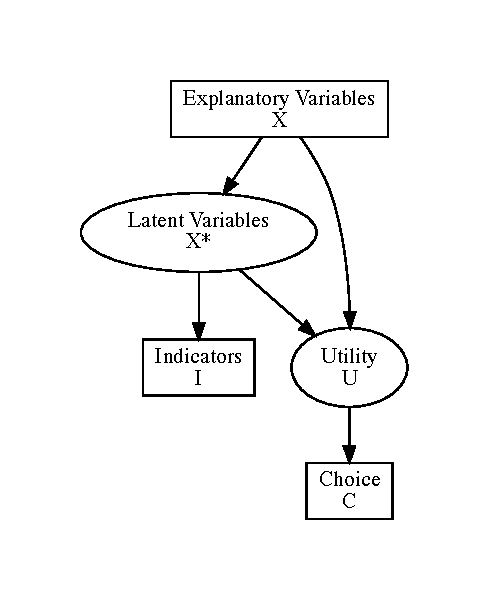
\includegraphics[width=0.35\textwidth]{iclv-causal-graph}
   \caption{Archetypical ICLV causal diagram}
   \label{fig:example-graph-iclv}
\end{figure}


Besides RUM models, causal graphs appear in the literature on Integrated Choice and Latent Variable (ICLV) models.
An example of an ICLV model is in Figure \ref{fig:example-graph-iclv}, based on Figure 5 of \citet{ben_2002_integration}.
As with RUM models, ICLV causal graphs represent assumptions about the choice process.
Here concern typically centers around unobserved mediators.
These unobserved variables cause the outcome and are caused by one's observed covariates.
Omitting such mediators leads to models that misrepresent the assumed choice process.
As a result, researchers care deeply about ICLV models that avoid these behavioral misrepresentations.

\begin{figure}
   \centering
   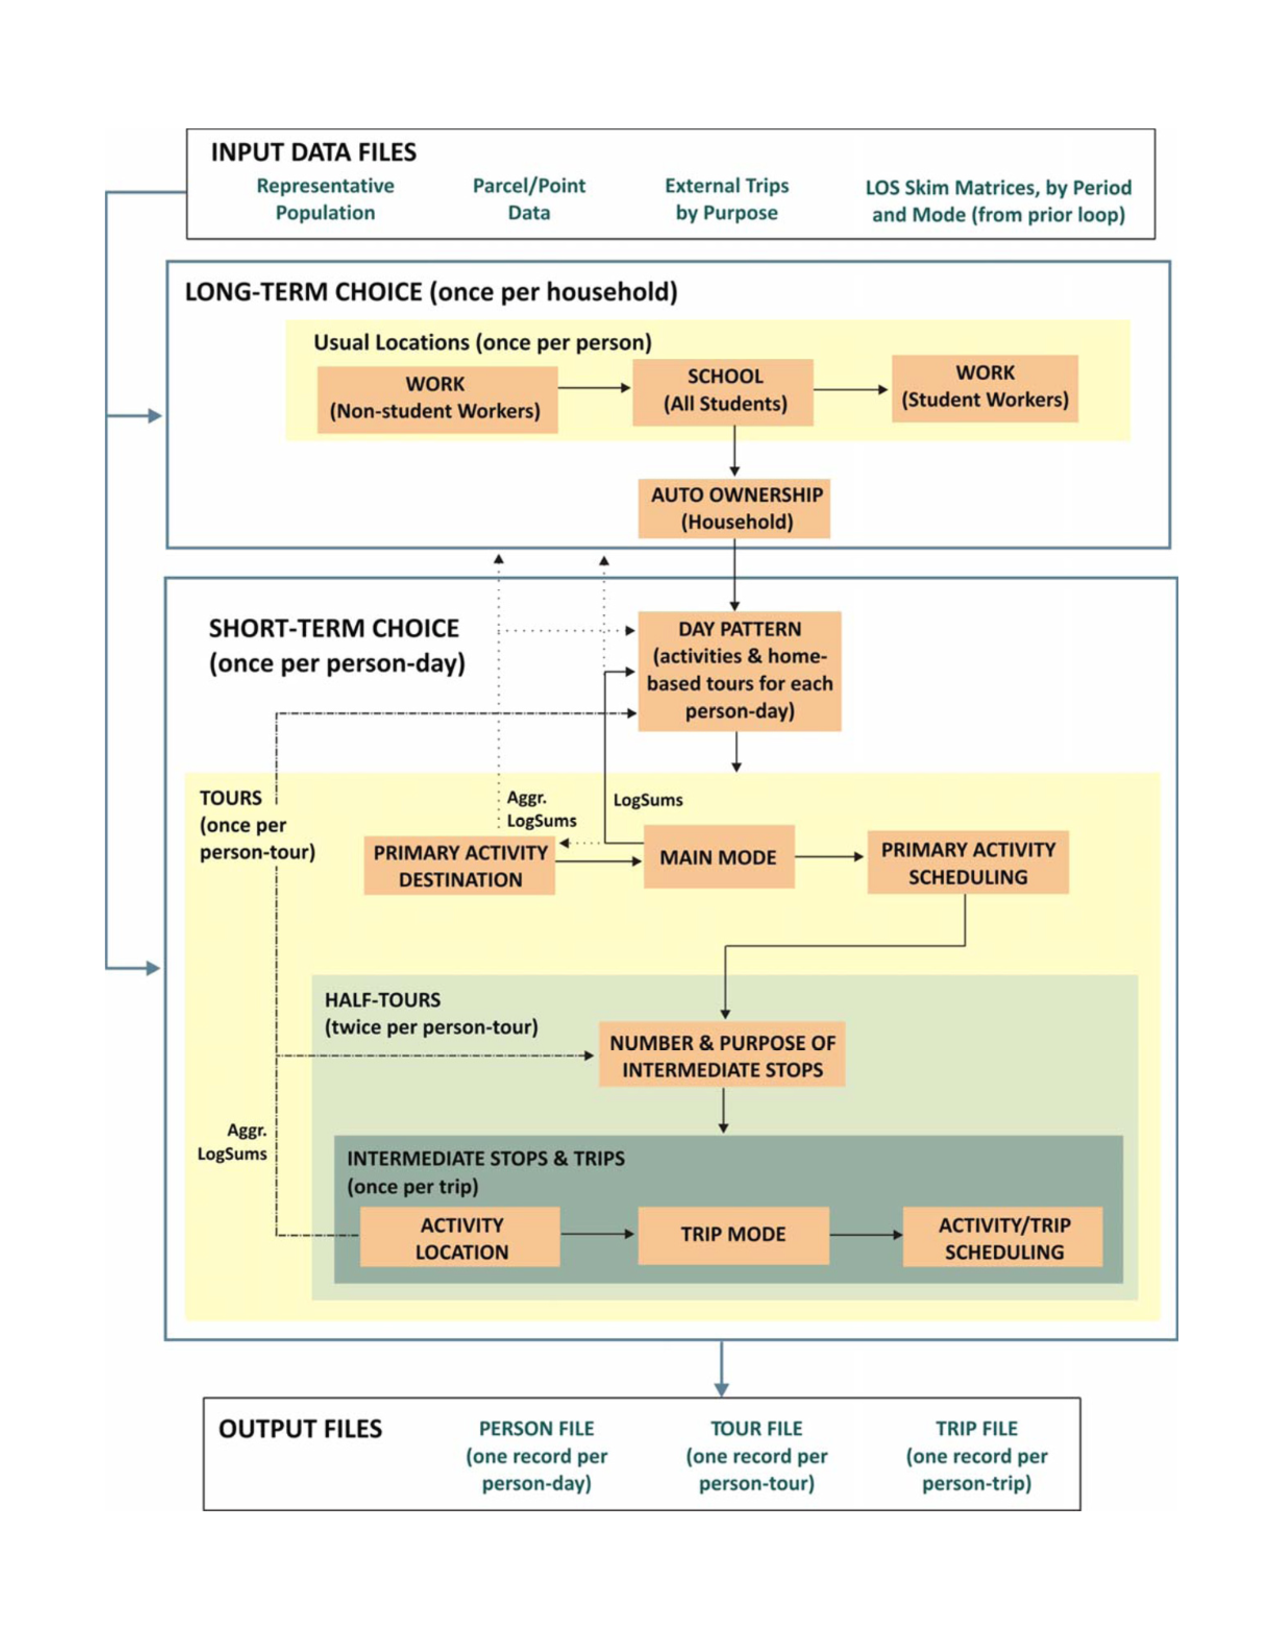
\includegraphics[width=0.5\textwidth]{daysim-model-graph}
   \caption{Archetypical causal diagram for activity-based models}
   \label{fig:example-graph-abm}
\end{figure}

Finally, consider activity based travel demand models (ABM).
These models often come with a causal diagram that depicts the interrelations between the outcomes in the model.
E.g., household location choice, destination choice, travel mode choice, departure time choice, route choice etc.
For example, see Figure \ref{fig:example-graph-abm}, from \citet[Fig. 2]{bradley_2010_sacsim}.
The purpose of these graphs is to explain the structure of the entire system of outcome models.

In particular, ABM diagrams highlight two sets of researcher assumptions.
They detail the researcher's beliefs about which choices, i.e. outcomes, precede others.
For instance, work location choice preceding auto-ownership choice.
ABM diagrams also detail which downstream choices partially cause which preceding ones.
For example, considerations about one's travel mode choice influences one's daily activity choices.
This happens even though the activity choices precede the travel mode choices.

Two main features distinguish RUM, ICLV, and ABM graphs from the causal graphs of \citet{pearl_1995_causal}.
First, causal graphs in choice modelling traditionally ignore relations between the explanatory variables.
Typically, choice modelling causal graphs show all explanatory variables together as a monolith.
The relationships between explanatory variables is often not specified.
Even worse, researchers may tacitly treat the variables as if they are jointly independent.
In the language used by a large group of causal inference scholars, econometric causal diagrams ignore the treatment assignment mechanism.

Secondly, causal graphs in choice modelling papers are purely didactic.
They convey how choice modellers perceive the world and the choice generation process.
However, they are seldom treated as a model themselves.
In particular, choice modellers rarely test the predictions of causal graphs.
In doing so, we underuse causal implications such as statistical independence.
Worse, we possibly violate these implications with great frequency.
Such actions ignore the efforts from causal inference in computer science.
There, researchers stress using their data to test the implications of their causal graphs.

In conclusion, choice modellers have long made use of causal graphs.
In select contexts, causal graphs convey causal assumptions about choice processes.
Thus far, however, our field has underutilized these tools.
We seldom use causal graphs to encode our assumptions about how our explanatory variables came to be.
Moreover, we do not routinely test causal graphs against empirical choice data.

These two issues are opportunities for choice modelling to gain from the insights and methods of causal inference scholars.
The rest of the chapter will focus on the following three topics.
How we can construct causal diagrams that pay attention to explanatory and outcome variables?
How we can test a given causal graph against one's data?
How can we deal with ``real-world'' graphs featuring unobserved confounding?
